\documentclass[12pt,a4paper]{article}
\usepackage[utf8]{inputenc}

% Format
\usepackage{layout}

% Font
\usepackage{MinionPro}
\input glyphtounicode
\pdfgentounicode=1
\usepackage{microtype}
\usepackage[super]{nth}
\usepackage{tfrupee}

% Language
\usepackage[british]{babel}

% References
\usepackage[nosectionbib, tocbib, unnumberedbib]{apacite}

% Figures
\usepackage{graphicx}
\usepackage{caption}    
\graphicspath{ {figures/} }

% Tables
\usepackage{booktabs}
\usepackage{tabularx}

% Commands
\newcommand{\pest}[4]{$ \text{Pr} (\text{``us''} | \text{#1}) = #2$, $[#3, #4]$}
\newcommand{\pdif}[4]{$ \Delta\text{Pr} (\text{``us''} | \text{#1}) = #2$, $[#3, #4]$}

\begin{document}

% Captions
\captionsetup[figure]{font={small},labelfont={it},labelformat={default}, labelsep=period}
\captionsetup[table]{font={small},labelfont={it},labelformat={default}, labelsep=period}

\begin{table}[h]
\caption[Participants by gender, age, nationality, religion, and caste]{Participants by gender, age, nationality, religion, and caste. Categories in \textit{italics} were excluded from the final sample. N/A marks missing responses.}
\centering
\figureversion{lining, tabular}
\small	
\begin{tabular}{llrr} \addlinespace \toprule
\multicolumn{2}{l}{Category} & $n$ & \% \\ \midrule \addlinespace 
Gender      & Woman      & 215 & 61 \\
            & Man & 121 & 34 \\
            & Other & 0 & 0 \\
            & N/A & 15 & 4 \\ \addlinespace \addlinespace
Age         & 18--20 & 1 & 0 \\
            & 21--23 & 254 & 72 \\
            & 24--26 &  77 & 22 \\
            & 27--29 &  10 &  3 \\
            & 30--32 &   1 &  0 \\
            & 33--35 &   0 &  0 \\
            & 36 or older & 1 & 0 \\ 
            & N/A & 7 & 2 \\ \addlinespace \addlinespace
Nationality & Indian & 339 & 97 \\
            & Other & 0 & 0 \\
            & N/A & 12 & 3 \\ \addlinespace \addlinespace
Religion    & Buddhism & 1 & 0 \\ 
            & Christianity & 11 & 3 \\ 
            & Hinduism & 297 & 85 \\ 
            & \textit{Islam} & \textit{27} & \textit{8} \\ 
            & Jainism & 8 & 2 \\ 
            & Other & 2 & 1 \\ 
            & N/A & 5 & 1 \\ \addlinespace \addlinespace
Caste       & General Caste & 104 & 30 \\ 
            & Other Backward Class & 143 & 41 \\ 
            & Scheduled Caste & 54 & 15 \\ 
            & Scheduled Tribe & 23 & 7 \\ 
            & \textit{Other / Not applicable} & \textit{20} & \textit{6} \\ 
            & \textit{N/A} & \textit{7} & \textit{2} \\ \addlinespace \midrule
Total       &   & 351 & 100 \\ \bottomrule
\end{tabular}
\label{tab:t1}
\end{table}

\begin{figure}
\centering
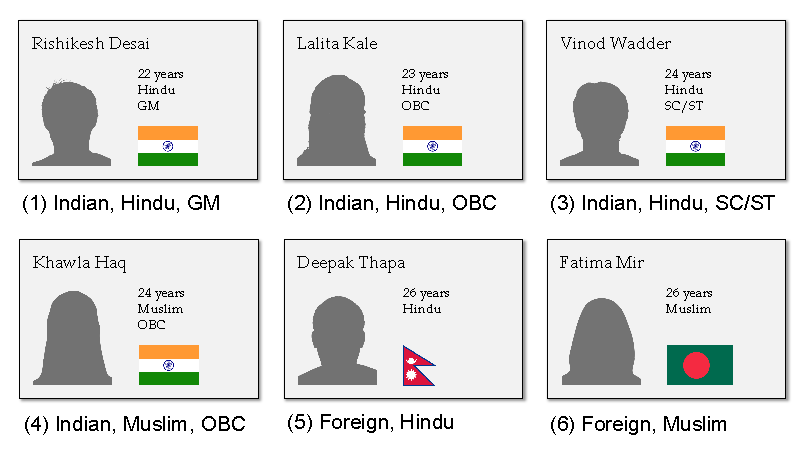
\includegraphics[scale=1]{../figures/figure-1}
\caption{Examples of targets used in the triple crossed-categorization task. Based on ratings in pilot study ($N = 26$), we selected the four most prototypical targets (out of fifty initial targets) for each of six plausible combinations of caste, religion, and nationality (for details, see Appendix~A). Each target showed a person's caste (GM = General Merit, OBC = Other Backward Class, SC/ST = Scheduled Caste/Scheduled Tribe), religion (Hindu, Muslim), and nationality (Indian, Nepali, Sri Lankan, Bangladeshi). Each target also showed the person's first and last name, age (21--26 years), and a silhouette corresponding to the person's gender (adapted from Ma, Correll \& Wittenbrink, 2015). Each target's age and silhouette, as well as the order in which the targets were presented, varied across sessions.}
\label{fig:f1}
\end{figure}

\begin{table}
\caption{}
\centering
\figureversion{lining, tabular}
\small	
\begin{tabularx}{\linewidth}{r@{~}rXrrrrr} \toprule
\# &  & Description & $\textit{ELPD}$ & $\textit{SE}$ & $\Delta\textit{ELPD}$ & $\textit{SE}$ & $\frac{\Delta\textit{ELPD}}{\textit{SE}}$ \\ \midrule 
0 &      & \ldots & -4262.5 & 33.0 & - & - & - \\
1 & vs 0 & \ldots & -3156.0 & 46.7 & 1106.6 & 42.7 & 25.9 \\
2 & vs 1 & \ldots & -3073.5 & 47.3 &   82.5 & 11.9 &  6.9 \\
3 & vs 2 & \ldots & -3068.1 & 47.4 &    5.4 &  3.4 &  1.6 \\ \midrule
4 & vs 2 & \ldots & . & . & . & . & . \\
5 & vs 4 & \ldots & . & . & . & . & . \\
6 & vs 5 & \ldots & . & . & . & . & . \\
7 & vs 2 & \ldots & . & . & . & . & . \\
\bottomrule
\end{tabularx}
\label{tab:t2}
\end{table}

\begin{figure}
\centering
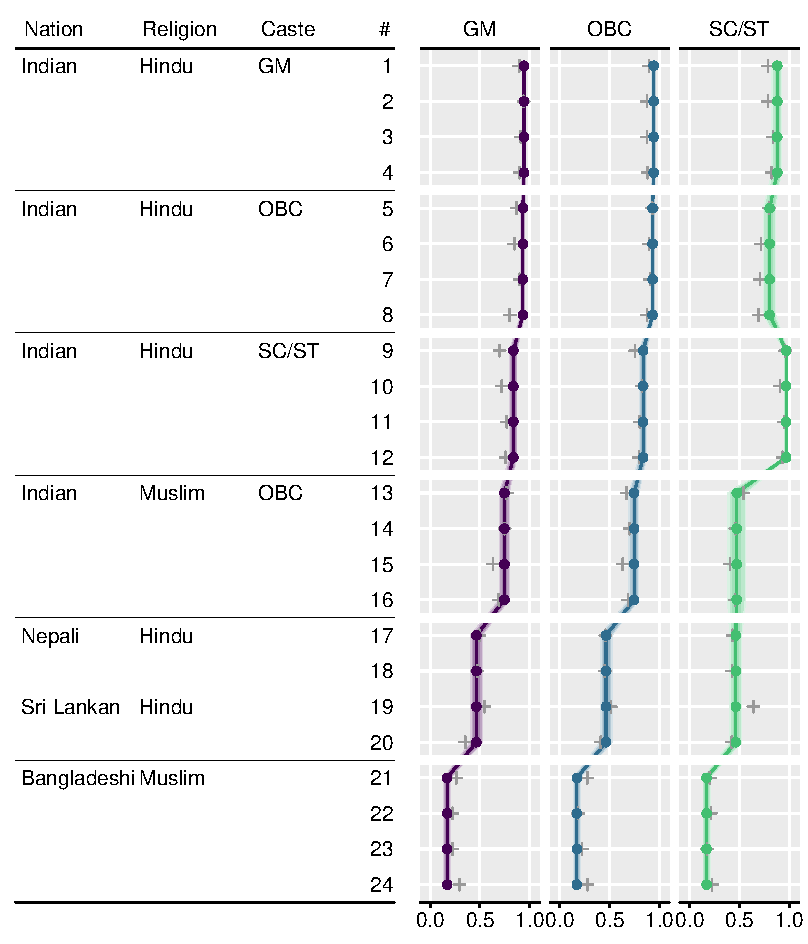
\includegraphics[scale=1]{../figures/figure-2}
\caption{
Estimated probability of participants categorizing a target as ``us'' versus ``not us'' by targets' nationality, religion, and caste (vertical), and participants' caste membership (horizontal). Dots (•) indicate the most likely \emph{estimate} for a given target's probability of being included in participants' ingroup (in Model~2, Table~\ref{tab:t2}), while the shaded ribbons encompass the 67\% (darkest shade), 89\%, and 97\% (lightest shade) most likely estimates of that probability. Pluses (+) indicate the \emph{observed} proportion of participants who included a given target in their ingroup. % Add sentence about posterior predictive checking.
}
\label{fig:f2}
\end{figure}

\begin{figure}
\centering
%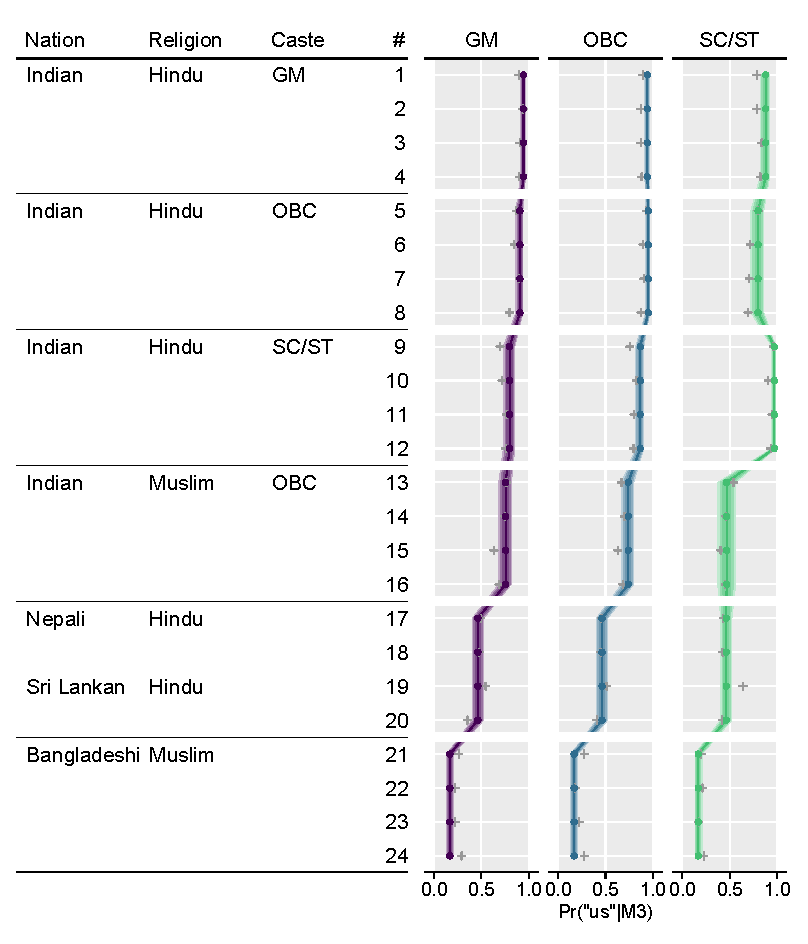
\includegraphics[scale=1]{../figures/figure-3}
\caption{Estimated probability of participants categorising a target as ``us'' versus ``not us'' as a function of the targets' group memberships (horizontal), the participants' group memberships (colour), and the reported amount of negative contact and outgroup friendship (in Model~5, Table~\ref{tab:t2}).}
\label{fig:f3}
\end{figure}

\begin{table}
\caption{}
\centering
\figureversion{lining, tabular}
\small	
\begin{tabularx}{\linewidth}{r@{~}rXrrrrrrr} \toprule
\# &  & Description & $R^2_\text{Q2}$ & $R^2_\text{Q3}$ & $\textit{ELPD}$ & $\textit{SE}$ & $\Delta\textit{ELPD}$ & $\textit{SE}$ & $\frac{\Delta\textit{ELPD}}{\textit{SE}}$ \\ \midrule 
0 &      & \ldots & . & . & . & . & . & . & . \\
1 & vs 0 & \ldots & . & . & . & . & . & . & . \\
2 & vs 1 & \ldots & . & . & . & . & . & . & . \\
3 & vs 2 & \ldots & . & . & . & . & . & . & . \\ \midrule
4 & vs 3 & \ldots & . & . & . & . & . & . & . \\
5 & vs 4 & \ldots & . & . & . & . & . & . & . \\
6 & vs 5 & \ldots & . & . & . & . & . & . & . \\
\bottomrule
\end{tabularx}
\label{tab:t3}
\end{table}

\end{document}